	\subsubsection{UC\theuccount-PG - Gitlab segnala la modifica di una issue al Producer Gitlab}
%	\begin{figure}[H]
%		\centering
%		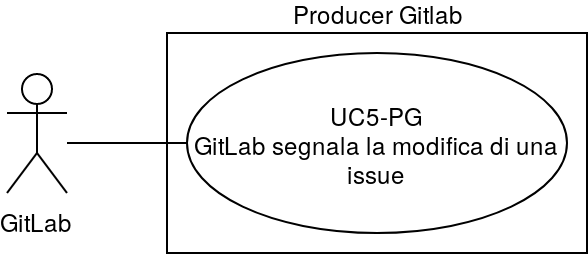
\includegraphics[width=0.5\textwidth]{img/casi_d'uso/UC5.png}\\
%		\caption{UC\theuccount-PG - Gitlab segnala la modifica di una issue al Producer Gitlab}
%	\end{figure}
	\begin{itemize}
		\item \textbf{Codice}: UC\theuccount-PG.
		\item \textbf{Titolo}: Gitlab segnala la modifica di una issue al Producer Gitlab.
		\item \textbf{Attori primari}: GitLab.
		\item \textbf{Descrizione}: GitLab segnala la modifica di una issue esistente tramite webhook a
		\newline \progetto.
		\item \textbf{Precondizione}: Viene modificata una issue già aperta su un
		progetto di GitLab da segnalare a \progetto.
		\item \textbf{Postcondizione}: il Producer GitLab riceve la segnalazione da GitLab.
		\item \textbf{Scenario principale}: 
		\begin{enumerate}
			\item Viene modificata una issue già esistente su GitLab
			\item GitLab procede all'invio della segnalazione di modifica issue al Producer GitLab
		\end{enumerate}
		
	\end{itemize}